\section{Background}
\subsection{About the OS}
QuarkTS is an open-source operating system that is built on top of a cooperative quasi-static scheduler. Its simplified kernel implements a specialized round-robin scheme using a linked-chain approach and an event-queue to provide true FIFO priority-scheduling.

\textbf{Why cooperative?}

Rather than having preemption,  tasks manage their own life-cycle. This bring significant benefits, fewer re-entrance problems are encountered, because tasks cannot be interrupted arbitrarily by other tasks, but only at positions permitted by the programmer, so you mostly do not need to worry about pitfalls of the concurrent approach(resource-sharing, races, deadlocks, etc...). 

\textbf{What is it made for?}

The design goal of QuarkTS is to achieve its stated functionality using a small, simple, and (most importantly) robust implementation to  make it suitable on resource-constrained microcontrollers, where a full-preemptive RTOS is an overkill and their inclusion adds unnecessary complexity to the firmware development. In addition with a state-machines support, co-routines, time control and the inter-task communication primitives, QuarkTS provides a modern environment to build stable and predictable event-driven multitasking embedded software. Their modularity and reliability make this OS a great choice to develop efficiently a wide range of applications in low-cost devices, including automotive controls, monitoring and Internet of Things.

\subsubsection{License}
QuarkTS is licensed under the MIT License. You may copy, distribute and modify the software without any restriction, including without limitation the rights to to use, copy, modify, merge, publish, distribute, sublicense, and/or sell copies of the OS, and to permit persons to whom the OS is furnished to do so. This OS is provided as is in the hope that it will be useful, but WITHOUT ANY WARRANTY; without even the implied warranty of MERCHANTABILITY or FITNESS FOR A PARTICULAR PURPOSE . 
For more details, see the MIT License in \cite{license}. 

\subsubsection{Hardware compatibility}
QuarkTS has no direct hardware dependencies, so it is portable to many platforms and C compilers. 
The following cores have been powered with QuarkTS successfully:
\begin{itemize}
    \item ARM cores(ATMEL, STM32, LPC, Kinetis, Nordic and others)
    \item 8Bit AVR, 8051, STM8
    \item HCS12, ColdFire, MSP430
    \item PIC (PIC24, dsPIC, 32MX, 32MZ)
\end{itemize}

\subsubsection{Development process and Coding standard}

QuarkTS is developed using a formal and rigorous process framed in compliance of the MISRA C 2012 and CERT coding standard guidelines and complemented with multiple static-analysis checks targered to safe critical applications.  

Simply using QuarkTS in an application, does not mean developers can make a claim related to the development process and compliance of the OS to any requirements or product specification, without first, following a recognized system wide conformance verification process. Conformance evidence must then be presented, audited and accepted by a recognized and relevant independent assessment organization. 
Without undergoing this process of due diligence, no claim can be made as to the suitability of QuarkTS to be used in any safety or otherwise commercially critical application.

Besides the previous information, the OS sets the following clarifications regarding coding policies and naming convention:

\begin{itemize}
    \item All the QuarkTS implementation follows the ANSI C99 standard strictly.
    \item Dynamic memory allocation is banned to conform the industry standards for safety-critical software: MISRA-C, DO178B, IEC 61508, ISO 26262 and so on.
    \item Because errors in string manipulation have long been recognized as a leading source of buffer overflows in C, a number of mitigation strategies have been devised. These include mitigation strategies designed to prevent buffer overflows from occurring and strategies designed to detect buffer overflows and securely recover without allowing the failure to be exploited.
    \item In line with MISRA guides and for portability between platforms, we use the \lstinline{stdint.h} with typedefs that indicate size and signedness in place of the basic types.
    \item In line with MISRA guides, unqualified standard \lstinline{char} and \lstinline{char *} types are only permitted to hold ASCII characters and strings respectively.    
    \item The \lstinline{_t} suffix its used to denote a type definition (i.e \lstinline{qBool_t, qTask_t, size_t, ...}).   
    \item Functions, macros, \lstinline{enum} values and data-types are prefixed \lstinline{q}. (i.e. \lstinline{qFunction}, \lstinline{qEnumValue}, \lstinline{QCONSTANT}, \lstinline{qType_t}, ...)
    \item Other than the pre-fix, most macros used for constants are written in all upper case.
    \item Almost all functions returns a boolean value of type \lstinline{qBool_t}, where a \lstinline{qTrue - 1u}  value indicates a successful procedure and \lstinline{qFalse - 0u}, the failure of the procedure.
\end{itemize}

\subsubsection{Memory usage}
As a quasi-static scheduler is implemented here, dynamic scheduling is not required and the assignment of tasks must be done before program execution begins.
The kernel is designed to allow unlimited tasks and kernel objects, but of course, the whole application will be constrained by the memory specifications of the embedded system. 
The kernel's memory footprint can be scaled down to contain only the features required for your application, typically 3.7 KBytes of code space and less than 1 KByte of data space. 

\begin{center}
\begin{tabular}{ |p{10cm}||p{1.5cm}|  }
    \hline
    \multicolumn{2}{|c|}{ \textbf{OS Memory Footprint} \scriptsize{(Measured in a 32bit MCU)}} \\
    \hline
    \textbf{Functionality} & \textbf{Size}\scriptsize{(bytes)}\\
    \hline
    Kernel, scheduler and task management& 2637\\
    A task node ({\lstinline!qTask_t!}) & 68\\
    Finite State-Machines(FSM) handling and related APIs& 314\\
    A FSM object ({\lstinline!qSM_t!}) & 84 \\
    A state object ({\lstinline!qSM_State_t!}) & 20 \\    
    STimers handling and related APIs & 258\\
    A STimer object ({\lstinline!qSTimer_t!})& 8\\
    Queues handling and related APIS & 544\\
    A queue object ({\lstinline!qQueue_t!}) & 28\\
    Memory management & 407\\
    A memory pool ({\lstinline!qMemMang_Pool_t!}) & 28 \\ 
    The AT Command Line Interface & 1724\\
    An AT-CLI instance ({\lstinline!qATCLI_t!})& 112\\
    An AT-CLI command object ({\lstinline!qATCLI_Command_t!})& 24\\
    Remaining utilities& 2980\\
    \hline
\end{tabular}
\end{center}

 \begin{tcolorbox}
 \HandRight Although the kernel does not use dynamically-allocated resources internally, the application writer can create an object in run-time using the safe-heap implementation provided by the memory management module, later described in section \ref{memmanagement}. Of course, additional checks must be performed to keep the solution safe.
 \end{tcolorbox}

\subsection{Timing approach}
The kernel implements a Time-Triggered Architecture (TTA)\cite{pont}, in which the tasks are triggered by comparing the corresponding task-time with a reference clock. The reference clock must be real-time and follow a monotonic behavior. Usually, all embedded systems can provide this kind of reference with a constant tick generated by a periodic background hardware-timer, typically, at 1Khz (1mS tick). 

For this, the kernel allows you to select the reference clock source among these two scenarios:

\begin{itemize}
    \item  When tick already provided: The reference is supplied by the Hardware Abstraction Layer (HAL) of the device.
        It is the simplest scenario and it occurs when the framework or SDK of the embedded system includes a HAL-API that obtains the time elapsed since the system starts, usually in milliseconds and taking a  32-bit counter variable.
    \item When the tick is not provided: The application writer should use bare-metal code to configure the device and feed the reference clock manually.
        Here, a hardware timer should raise an interrupt periodically. After the \textit{Interrupt Service Routine} (ISR) has been implemented using the platform-dependent code, the \lstinline{qClock_SysTick()} \index{\lstinline{qClock_SysTick}} API must be called inside. It is recommended that the reserved ISR should only be used by QuarkTS.
\end{itemize}

\subsection{Setting up the OS kernel : \texorpdfstring{\lstinline{qOS_Setup}}{qOS_Setup} } \label{settingupkernel}
 This function should be the first call to the OS APIs. \lstinline{qOS_Setup()} \index{\lstinline{qOS_Setup}} prepares the kernel instance, sets the reference clock, defines the \textit{Idle-Task} callback and allocates the stack for the internal queue.
\medskip 
 
\begin{lstlisting}[style=CStyle]
void qOS_Setup( const qGetTickFcn_t TickProvider, 
                const qTimingBase_t BaseTimming, 
                qTaskFcn_t IdleCallback )
\end{lstlisting}

\subsubsection*{Parameters}
\begin{itemize}
    \item \lstinline{TickProvider} : The function that provides the tick value. If the user application uses the \lstinline{qClock_SysTick()} from the ISR, this parameter can be \lstinline{NULL}. 
    
    Note: Function should take \lstinline{void} and return a 32bit unsigned integer.
    
    This argument must have this prototype : \lstinline{qUINT32_t TickProviderFcn(void)}
    \item \lstinline{BaseTimming} :This parameter specifies the ISR background timer period in seconds(floating-point format).
    
    \textit{Note} : This argument will be only available if \lstinline{Q_SETUP_TIME_CANONICAL} is set to zero(0).
    \item \lstinline{IdleCallback} : Callback function for the idle task. If not used, pass \lstinline{NULL} as argument.
\end{itemize}


\begin{tcolorbox}
\HandRight This call is mandatory and must be called once in the application main thread before any kind of interaction with the OS.
\end{tcolorbox}

\subsubsection*{Usage example:}
Scenario 1: When tick is already provided
\lstinputlisting[style=CStyle]{sec1scenario1.c}


Scenario 2: When the tick is not provided
\lstinputlisting[style=CStyle]{sec1scenario2.c}

\subsection{Tasks}
Like many operating systems, the basic unit of work is the task. Tasks can perform certain functions, which could require periodic or one-time execution, update of specific variables or waiting for specific events. Tasks also could be controlling specific hardware or be triggered by hardware interrupts. In the QuarkTS OS, a task is seen as a node concept that links together:

\begin{itemize}
    \item Program code performing specific task activities (callback function)
    \item Execution interval (time)
    \item Number of execution (iterations)
    \item Event-based data
\end{itemize}

The OS  uses a \textit{Task Control Block} (TCB) to represent each task, storing essential information about task management and execution. Part of this information also includes \textit{link-pointers} that allows it to be part of one of the lists available in the Kernel Control Block (KCB).

\begin{figure}[H]
    \centering
    \tikzset{every picture/.style={line width=0.75pt}} %set default line width to 0.75pt        
    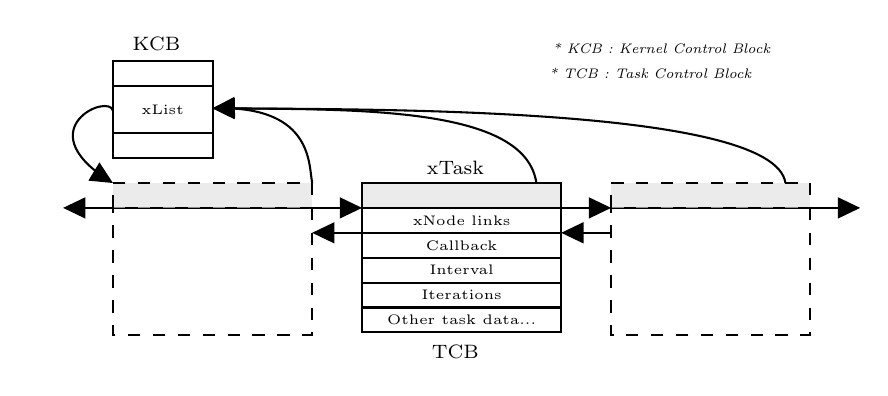
\begin{tikzpicture}[x=0.75pt,y=0.75pt,yscale=-1,xscale=1,scale=1.2]
        \draw   (220,99) -- (300,99) -- (300,109) -- (220,109) -- cycle ;
        \draw  [fill=lightgray!50  ,fill opacity=0.62 ] (220,79) -- (300,79) -- (300,89) -- (220,89) -- cycle ;
        \draw    (220,99) -- (203,99) ;
        \draw [shift={(200,99)}, rotate = 360] [fill=black][line width=0.08]  [draw opacity=0] (8.93,-4.29) -- (0,0) -- (8.93,4.29) -- cycle;
        \draw   (220,109) -- (300,109) -- (300,119) -- (220,119) -- cycle ;
        \draw   (220,119) -- (300,119) -- (300,129) -- (220,129) -- cycle ;
        \draw  [dash pattern={on 4.5pt off 4.5pt}] (320,89) -- (400,89) -- (400,140) -- (320,140) -- cycle ;
        \draw  [fill=lightgray!50  ,fill opacity=0.62 ][dash pattern={on 4.5pt off 4.5pt}] (320,79) -- (400,79) -- (400,89) -- (320,89) -- cycle ;
        \draw   (220,129) -- (300,129) -- (300,139) -- (220,139) -- cycle ;
        \draw  [dash pattern={on 4.5pt off 4.5pt}] (120,89) -- (200,89) -- (200,140) -- (120,140) -- cycle ;
        \draw  [fill=lightgray!50  ,fill opacity=0.62 ][dash pattern={on 4.5pt off 4.5pt}] (120,79) -- (200,79) -- (200,89) -- (120,89) -- cycle ;
        \draw    (200,89) -- (217,89) ;
        \draw [shift={(220,89)}, rotate = 180] [fill=black][line width=0.08]  [draw opacity=0] (8.93,-4.29) -- (0,0) -- (8.93,4.29) -- cycle;
        \draw   (220,89) -- (300,89) -- (300,99) -- (220,99) -- cycle ;
        \draw    (320,99) -- (303,99) ;
        \draw [shift={(300,99)}, rotate = 360] [fill=black][line width=0.08]  [draw opacity=0] (8.93,-4.29) -- (0,0) -- (8.93,4.29) -- cycle;
        \draw    (300,89) -- (317,89) ;
        \draw [shift={(320,89)}, rotate = 180] [fill=black][line width=0.08]  [draw opacity=0] (8.93,-4.29) -- (0,0) -- (8.93,4.29) -- cycle;
        \draw    (120,89) -- (103,89) ;
        \draw [shift={(100,89)}, rotate = 360] [fill=black][line width=0.08]  [draw opacity=0] (8.93,-4.29) -- (0,0) -- (8.93,4.29) -- cycle;
        \draw    (400,89) -- (417,89) ;
        \draw [shift={(420,89)}, rotate = 180] [fill=black][line width=0.08]  [draw opacity=0] (8.93,-4.29) -- (0,0) -- (8.93,4.29) -- cycle;
        \draw   (120,30) -- (160,30) -- (160,40) -- (120,40) -- cycle ;
        \draw   (120,40) -- (160,40) -- (160,59) -- (120,59) -- cycle ;
        \draw   (120,59) -- (160,59) -- (160,69) -- (120,69) -- cycle ;
        \draw    (290,79) .. controls (285.57,48.04) and (217.59,49.52) .. (162.51,49.02) ;
        \draw [shift={(160,49)}, rotate = 360.59] [fill=black][line width=0.08]  [draw opacity=0] (8.93,-4.29) -- (0,0) -- (8.93,4.29) -- cycle;
        \draw    (200,79) .. controls (198.54,71.76) and (200.4,48.76) .. (162.96,48.94) ;
        \draw [shift={(160,49)}, rotate = 357.98] [fill=black][line width=0.08]  [draw opacity=0] (8.93,-4.29) -- (0,0) -- (8.93,4.29) -- cycle;
        \draw    (390,79) .. controls (385.57,48.04) and (220.56,49.52) .. (162.57,49.02) ;
        \draw [shift={(160,49)}, rotate = 360.59] [fill=black][line width=0.08]  [draw opacity=0] (8.93,-4.29) -- (0,0) -- (8.93,4.29) -- cycle;
        \draw    (120,50) .. controls (118.54,42.76) and (86.18,56.84) .. (117.47,77.41) ;
        \draw [shift={(120,79)}, rotate = 211.12] [fill=black][line width=0.08]  [draw opacity=0] (8.93,-4.29) -- (0,0) -- (8.93,4.29) -- cycle;
        \draw (260,104) node  [font=\tiny] [align=left] {Callback};
        \draw (260,114) node  [font=\tiny] [align=left] {Interval};
        \draw (260,124) node  [font=\tiny] [align=left] {Iterations};
        \draw (260,134) node  [font=\tiny] [align=left] {Other task data...};
        \draw (257.5,147) node  [font=\scriptsize] [align=left] {TCB};
        \draw (260,94) node  [font=\tiny] [align=left] {xNode links};
        \draw (137.5,23) node  [font=\scriptsize] [align=left] {KCB};
        \draw (140,49.5) node  [font=\tiny] [align=left] {xList};
        \draw (257.5,73) node  [font=\scriptsize] [align=left] {xTask};
        \draw (340.5,25) node  [font=\tiny] [align=left] {\textit{* KCB : Kernel Control Block}};
        \draw (336,35) node  [font=\tiny] [align=left] {\textit{* TCB : Task Control Block}};
    \end{tikzpicture}
\caption{Task node illustration}
\label{fig:tasklist}
\end{figure}

Each task performs its activities via a callback function and each of them is responsible for supporting cooperative multitasking by being “good neighbors”, i.e., running their callback methods quickly in a non-blocking way and releasing control back to the scheduler as soon as possible (returning). 
\medskip

Every task node, must be defined using the \lstinline{qTask_t} \index{\lstinline{qTask_t}} data-type and the callback is defined as a function that returns \lstinline{void} and takes a \lstinline{qEvent_t} data structure as its only parameter (This input argument can be used later to get event information, see section \ref{eventdata}).
\medskip

\begin{lstlisting}[style=CStyle]
qTask_t UserTask;
void UserTask_Callback( qEvent_t eventdata ){
    /* TODO : Task code */
}
\end{lstlisting}

\begin{tcolorbox}
\ArrowBoldDownRight \textit{Note} : All tasks in QuarkTS must ensure their completion to return the CPU control back to the scheduler, otherwise, the scheduler will hold the execution-state for that task, preventing the activation of other tasks.
\end{tcolorbox}

\subsubsection{The idle task}
Its a special task loaded by the OS scheduler when there is nothing else to do (no task in the whole scheme has reached the ready state). The idle task is already hard-coded into the kernel, ensuring that at least, one task is able to run. Additionally, the OS setup this task with the lowest possible priority to ensure that does not use any CPU time if there are higher priority application tasks able to run.
\medskip
The idle task doesn't perform any active functions, but the user can decide if it should perform some activities defining a callback function for it. This could be done at the beginning of the kernel setup (as seen in section \ref{settingupkernel} with \lstinline{qOS_Setup()}) or in run-time with \lstinline{qOS_Set_IdleTask()} \index{\lstinline{qOS_Set_IdleTask}}.
\medskip

\begin{lstlisting}[style=CStyle]
void qOS_Set_IdleTask(qTaskFcn_t Callback)
\end{lstlisting}

Of course, the callback must follow the same function prototype for tasks.
\medskip

\begin{tcolorbox}
\HandRight To disable the idle-task activities, a \lstinline{NULL} should be passed as argument.
\end{tcolorbox}

\subsubsection{Adding tasks to the scheme : \lstinline{qOS_Add_Task} } \label{addtask}
After setting up the kernel with \lstinline{qOS_Setup()}, the user can proceed to deploy the multitasking application by adding tasks. If the task node and their respective callback is already defined, the task can be added to the scheme using \lstinline{qOS_Add_Task()} \index{\lstinline{qOS_Add_Task}}. This API can schedule a task to run every \lstinline{Time} seconds, \lstinline{nExecutions} times and executing \lstinline{CallbackFcn} method on every pass.
\medskip

\begin{lstlisting}[style=CStyle]
qBool_t qOS_Add_Task( qTask_t * const Task, qTaskFcn_t CallbackFcn, 
                      qPriority_t Priority, qTime_t Time, 
                      qIteration_t nExecutions, qState_t InitialState, 
                      void* arg )
\end{lstlisting}

\subsubsection*{Parameters}
\begin{itemize}
    \item \lstinline{Task} : A pointer to the task node. 
    \item \lstinline{CallbackFcn} : A pointer to a void callback method with a \lstinline{qEvent_t} parameter as input argument..
    \item \lstinline{Priority} : The priority value. [0(min) - \lstinline{Q_PRIORITY_LEVELS}(max)]
    \item \lstinline{Time} : Execution interval defined in seconds (floating-point format). For immediate execution use the  \lstinline{qTimeImmediate} definition. 
    \item \lstinline{nExecutions} : Number of task executions (Integer value). For indefinite execution  use \lstinline{qPeriodic} or the \lstinline{qIndefinite} definition. 
    \item \lstinline{InitialState} : Specifies the initial operational state of the task (\lstinline{qEnabled}, \lstinline{qDisabled}, \lstinline{qAsleep} or \lstinline{qAwake}(implies \lstinline{qEnabled})).
    \item \lstinline{arg} - Represents the task argument. This argument must be passed by reference and cast to \lstinline{(void *)}. 
\end{itemize}

\subsubsection*{Return value}
\lstinline{qTrue} if the task was successfully added the scheme. Otherwise returns \lstinline{qFalse}.

\subsubsection*{Caveats}
\begin{enumerate}
    \item A task with \lstinline{Time} argument defined in \lstinline{qTimeImmediate}, will always get the \textit{qReady} state in every scheduling cycle, as consequence, the idle task will never gets dispatched.
    \item Tasks do not remember the number of iteration set initially by the \lstinline{nExecutions} argument. After the iterations are done, the internal iteration counter decreases until reach the zero. If another set of iterations is needed, the user should set the number of iterations again and resume the task explicitly. 
    \item Tasks that performed all their iterations, put their own state to \lstinline{qDisabled}. Asynchronous triggers do not affect the iteration counter.
    \item The \lstinline{arg} parameter can be used as storage pointer, so, for multiple data, create a structure with the required members and pass a pointer to that structure.
\end{enumerate}

\noindent\hrulefill

Invoking \lstinline{qOS_Add_Task()}  is the most generic way to adding tasks to the scheme, supporting a mixture of time-triggered and event-triggered tasks, however, additional simplified API functions are also provided to add specific purpose tasks:
\begin{itemize}
    \item Event-triggered only tasks $\rightarrow$ \lstinline{qOS_Add_EventTask()}
    \item State-machine tasks $\rightarrow$ \lstinline{qOS_Add_StateMachineTask()}. See section \ref{statemachinetask}.
    \item AT Command Line Interface tasks $\rightarrow$ \lstinline{qOS_Add_ATCLITask()}. See section \ref{runningparser}.
\end{itemize}


\subsubsection{Event-triggered tasks}
An event-triggered task reacts asynchronously to the occurrence of events in the system, such as external interrupts or changes in the available resources. 

The API \lstinline{qOS_Add_EventTask()} \index{\lstinline{qOS_Add_EventTask}} is intended to add this kind of tasks, keeping it in a \textit{qSuspended} state. Only asynchronous events followed by their priority value dictates when a task can change to the \textit{qRunning} state. 
\medskip


\begin{lstlisting}[style=CStyle]
qBool_t qOS_Add_EventTask( qTask_t * const Task, qTaskFcn_t CallbackFcn, 
                           qPriority_t Priority, void* arg)
\end{lstlisting}

As seen above, arguments related to timing and iterations parameters are dispensed and the only required arguments become minimal, just needing:  \lstinline{CallbackFcn}, \lstinline{Priority} and the related task arguments \lstinline{arg}.

\subsubsection{Removing a task : \lstinline{qOS_Remove_Task}}
As expected, the API \index{\lstinline{qOS_Remove_Task}}removes the task from the scheduling scheme.  This means the task node will be disconnected from the kernel chain, preventing additional overhead provided by the scheduler when it does checks over it and course, preventing from running. 
\medskip

\begin{lstlisting}[style=CStyle]
qBool_t qOS_Remove_Task( qTask_t * const Task )
\end{lstlisting}

\subsubsection*{Caveats:}
Task nodes are variables like any other. They allow your application code to reference a task, but there is no link back the other way and the kernel doesn't know anything about the variables, where the variable is allocated (stack, global, static, etc.) or how many copies of the variable you have made, or even if the variable still exists.  So the \lstinline{qOS_Remove_Task()} API cannot automatically free the resources allocated by the variable. 
If the task node has been dynamically allocated, the application writer it's responsible to free the memory block after a removal call.


\subsection{Running the OS : \lstinline{qOS_Run}}
After preparing the multitasking environment for your application, a call to \lstinline{qOS_Run()} \index{\lstinline{qOS_Run}} is required to execute the scheduling scheme.
This function is responsible to run the following OS main components:
\begin{itemize}
    \item \textbf{The Scheduler} : Select the tasks to be submitted into the system and decide with of them are able to run.
    \item \textbf{The Dispatcher} : When the scheduler completes its job of selecting ready tasks, it is the dispatcher which takes that task to the running state. This procedure gives a task control over the CPU after it has been selected by the scheduler. This involves the following:
    \begin{itemize}
        \item Preparing the resources before the task execution
        \item Execute the task activities (via the callback function)
        \item Releasing the resources after the task execution 
    \end{itemize}
\end{itemize}

The states involved in the interaction between the scheduler and dispatcher are described in the section that follows.
\medskip

\begin{tcolorbox}
\ArrowBoldDownRight \textit{Note}: After calling \lstinline{qOS_Run()}, the OS scheduler will now be running, and the following line should never be reached, however, the user can optionally release it explicitly with \lstinline{qOS_Scheduler_Release()} API function.
\end{tcolorbox}

\subsubsection{Releasing the scheduler: \lstinline{qOS_Scheduler_Release} }
This functionality must be enabled from the \lstinline{Q_ALLOW_SCHEDULER_RELEASE} macro.
This API \index{\lstinline{qOS_Scheduler_Release}} stop the kernel scheduling. In consequence, the main thread will continue after the \lstinline{qOS_Run()} call. 

Although producing this action is not a typical desired behavior in any application, it can be used to handle a critical exception.

When used, the release will take place after the current scheduling cycle finish. The kernel can optionally include a release callback function that can be configured to get called if the scheduler is released. 
Defining the release callback,  will help to take actions over the exception that caused the release action. To perform a release action, the \lstinline{qOS_Set_SchedulerReleaseCallback()} \index{\lstinline{qOS_Set_SchedulerReleaseCallback}} API should be used. 
\medskip

\begin{lstlisting}[style=CStyle]
void qOS_Set_SchedulerReleaseCallback( qTaskFcn_t Callback )
\end{lstlisting}

\begin{tcolorbox}
\HandRight When a scheduler release is performed, resources are not freed. After released, the application can invoke the \lstinline{qOS_Run()} again to resume the scheduling activities.
\end{tcolorbox}

\subsection{Global states and scheduling rules}

A task can be in one of the four global states: \textit{qRunning}, \textit{qReady}, \textit{qSuspended} or \textit{qWaiting}. Each of these states is tracked implicitly by putting the task in one of the associated kernel lists. 

These global states are described below:

\begin{figure}[H]
    \centering
    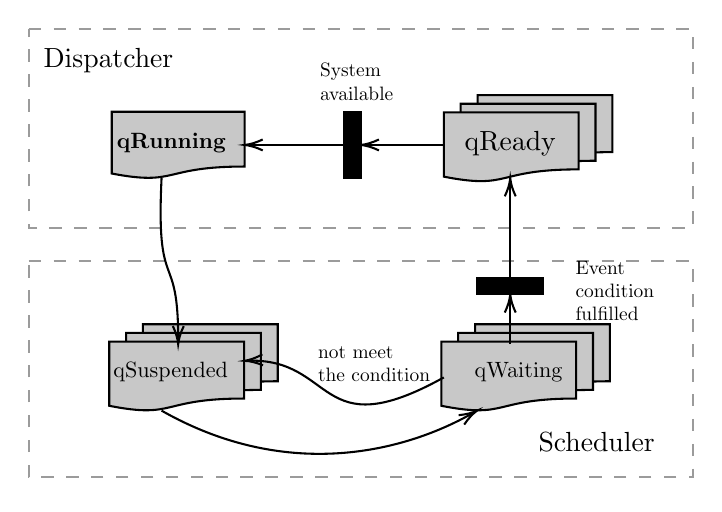
\begin{tikzpicture}[x=0.75pt,y=0.75pt,yscale=-1,xscale=1,scale=0.8]
        \draw  [fill={rgb, 255:red, 200; green, 200; blue, 200 }  ,fill opacity=1 ] (378.8,188) -- (460,188) -- (460,222.32) .. controls (409.25,222.32) and (419.4,234.7) .. (378.8,226.69) -- cycle ; \draw  [fill={rgb, 255:red, 200; green, 200; blue, 200 }  ,fill opacity=1 ] (368.65,193.2) -- (449.85,193.2) -- (449.85,227.52) .. controls (399.1,227.52) and (409.25,239.9) .. (368.65,231.89) -- cycle ; \draw  [fill={rgb, 255:red, 200; green, 200; blue, 200 }  ,fill opacity=1 ] (358.5,198.4) -- (439.7,198.4) -- (439.7,232.72) .. controls (388.95,232.72) and (399.1,245.1) .. (358.5,237.09) -- cycle ;
        \draw  [fill={rgb, 255:red, 200; green, 200; blue, 200 }  ,fill opacity=1 ] (178.8,188) -- (260,188) -- (260,222.32) .. controls (209.25,222.32) and (219.4,234.7) .. (178.8,226.69) -- cycle ; \draw  [fill={rgb, 255:red, 200; green, 200; blue, 200 }  ,fill opacity=1 ] (168.65,193.2) -- (249.85,193.2) -- (249.85,227.52) .. controls (199.1,227.52) and (209.25,239.9) .. (168.65,231.89) -- cycle ; \draw  [fill={rgb, 255:red, 200; green, 200; blue, 200 }  ,fill opacity=1 ] (158.5,198.4) -- (239.7,198.4) -- (239.7,232.72) .. controls (188.95,232.72) and (199.1,245.1) .. (158.5,237.09) -- cycle ;
        \draw  [fill={rgb, 255:red, 200; green, 200; blue, 200 }  ,fill opacity=1 ] (380.3,50) -- (461.5,50) -- (461.5,84.32) .. controls (410.75,84.32) and (420.9,96.7) .. (380.3,88.69) -- cycle ; \draw  [fill={rgb, 255:red, 200; green, 200; blue, 200 }  ,fill opacity=1 ] (370.15,55.2) -- (451.35,55.2) -- (451.35,89.52) .. controls (400.6,89.52) and (410.75,101.9) .. (370.15,93.89) -- cycle ; \draw  [fill={rgb, 255:red, 200; green, 200; blue, 200 }  ,fill opacity=1 ] (360,60.4) -- (441.2,60.4) -- (441.2,94.72) .. controls (390.45,94.72) and (400.6,107.1) .. (360,99.09) -- cycle ;
        \draw  [color={rgb, 255:red, 155; green, 155; blue, 155 }  ,draw opacity=1 ][dash pattern={on 4.5pt off 4.5pt}] (110,10) -- (510,10) -- (510,130) -- (110,130) -- cycle ;
        \draw  [fill={rgb, 255:red, 200; green, 200; blue, 200 }  ,fill opacity=1 ] (160,60) -- (240,60) -- (240,93) .. controls (190,93) and (200,104.9) .. (160,97.2) -- cycle ;
        \draw  [color={rgb, 255:red, 155; green, 155; blue, 155 }  ,draw opacity=1 ][dash pattern={on 4.5pt off 4.5pt}] (110,150) -- (510,150) -- (510,280) -- (110,280) -- cycle ;
        \draw    (360,220) .. controls (283.27,262.57) and (295.25,208.11) .. (241.64,209.93) ;
        \draw [shift={(240,210)}, rotate = 356.90999999999997] [color={rgb, 255:red, 0; green, 0; blue, 0 }  ][line width=0.75]    (10.93,-3.29) .. controls (6.95,-1.4) and (3.31,-0.3) .. (0,0) .. controls (3.31,0.3) and (6.95,1.4) .. (10.93,3.29);
        \draw    (190,240) .. controls (266.73,283.56) and (338.06,264.39) .. (378.78,240.72) ;
        \draw [shift={(380,240)}, rotate = 509.35] [color={rgb, 255:red, 0; green, 0; blue, 0 }  ][line width=0.75]    (10.93,-3.29) .. controls (6.95,-1.4) and (3.31,-0.3) .. (0,0) .. controls (3.31,0.3) and (6.95,1.4) .. (10.93,3.29)   ;
        \draw  [fill={rgb, 255:red, 0; green, 0; blue, 0 }  ,fill opacity=1 ] (420,160) -- (380,160) -- (380,170) -- (420,170) -- cycle ;
        \draw  [fill={rgb, 255:red, 0; green, 0; blue, 0 }  ,fill opacity=1 ] (310,60) -- (300,60) -- (300,100) -- (310,100) -- cycle ;
        \draw    (400,200) -- (400,172) ;
        \draw [shift={(400,170)}, rotate = 450] [color={rgb, 255:red, 0; green, 0; blue, 0 }  ][line width=0.75]    (10.93,-3.29) .. controls (6.95,-1.4) and (3.31,-0.3) .. (0,0) .. controls (3.31,0.3) and (6.95,1.4) .. (10.93,3.29)   ;
        \draw    (400,160) -- (400,102) ;
        \draw [shift={(400,100)}, rotate = 450] [color={rgb, 255:red, 0; green, 0; blue, 0 }  ][line width=0.75]    (10.93,-3.29) .. controls (6.95,-1.4) and (3.31,-0.3) .. (0,0) .. controls (3.31,0.3) and (6.95,1.4) .. (10.93,3.29)   ;
        \draw    (360,80) -- (312,80) ;
        \draw [shift={(310,80)}, rotate = 360] [color={rgb, 255:red, 0; green, 0; blue, 0 }  ][line width=0.75]    (10.93,-3.29) .. controls (6.95,-1.4) and (3.31,-0.3) .. (0,0) .. controls (3.31,0.3) and (6.95,1.4) .. (10.93,3.29)   ;
        \draw    (300,80) -- (242,80) ;
        \draw [shift={(240,80)}, rotate = 360] [color={rgb, 255:red, 0; green, 0; blue, 0 }  ][line width=0.75]    (10.93,-3.29) .. controls (6.95,-1.4) and (3.31,-0.3) .. (0,0) .. controls (3.31,0.3) and (6.95,1.4) .. (10.93,3.29)   ;
        \draw    (190,100) .. controls (186.54,172.27) and (200.22,140.65) .. (200.01,198.23) ;
        \draw [shift={(200,200)}, rotate = 270.48] [color={rgb, 255:red, 0; green, 0; blue, 0 }  ][line width=0.75]    (10.93,-3.29) .. controls (6.95,-1.4) and (3.31,-0.3) .. (0,0) .. controls (3.31,0.3) and (6.95,1.4) .. (10.93,3.29)   ;
        \draw (196,79) node  [scale=0.8, align=left] {\textbf{qRunning}};
        \draw (195.5,217) node [scale=0.8] [align=left] {qSuspended};
        \draw (405,217) node [scale=0.8] [align=left] {qWaiting};
        \draw (400,79) node [scale=1] [align=left] {qReady};
        \draw (158,29) node  [align=left] {Dispatcher};
        \draw (452,259) node  [align=left] {Scheduler};
        \draw (307.5,42) node [scale=0.7] [align=left] {System \\available};
        \draw (318,212) node [scale=0.7] [align=left] {not meet\\the condition};
        \draw (463,168) node [scale=0.7] [align=left] {Event\\condition\\fulfilled};
    \end{tikzpicture}
    \caption{Task global states}
    \label{fig:scheduler_states}
\end{figure}

\begin{itemize}
    \item \textbf{qWaiting} : The task cannot run because the conditions for running are not in place. 
    \item \textbf{qReady} : The task has completed preparations for running, but cannot run because a task with a higher precedence is running.
    \item \textbf{qRunning} : The task is currently being executed.
    \item \textbf{qSuspended} : The task doesn't take part in what is going on. Normally this state is taken after the \textit{qRunning} state or when the task doesn't reach the \textit{qReady} state.
\end{itemize}

\begin{figure}[H]
    \centering
    \tikzset{every picture/.style={line width=0.75pt}} %set default line width to 0.75pt        
    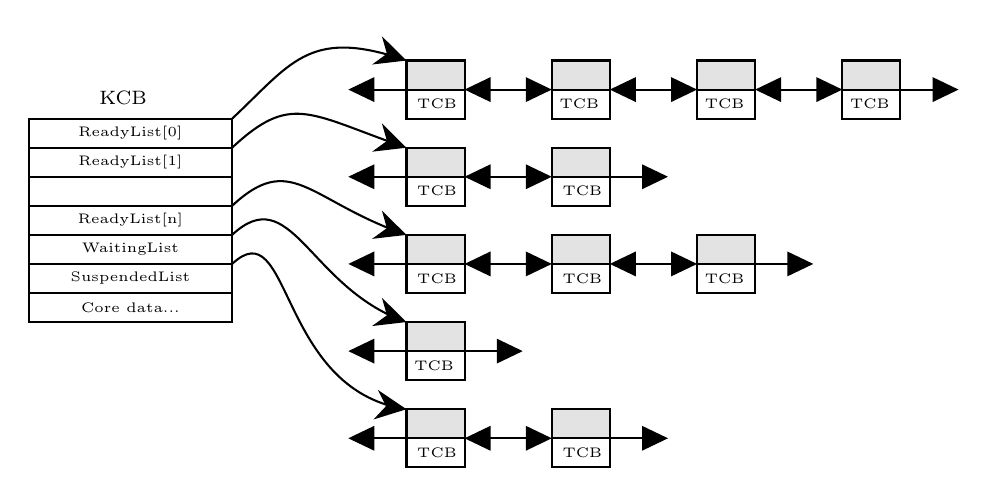
\begin{tikzpicture}[x=0.75pt,y=0.75pt,yscale=-1,xscale=1, scale=1.4]
        
        \foreach \x in {30,40,...,80}{
            \draw   (70,\x) -- (140,\x) -- (140,\x+10) -- (70,\x+10) -- cycle ;
        }
        
        \draw   (70,90) -- (140,90) -- (140,100) -- (70,100) -- cycle ;
        \draw   (200,10) -- (220,10) -- (220,30) -- (200,30) -- cycle ;
        \draw   (250,10) -- (270,10) -- (270,30) -- (250,30) -- cycle ;
        \draw  [fill={rgb, 255:red, 210; green, 210; blue, 210 }  ,fill opacity=0.62 ] (200,10) -- (220,10) -- (220,20) -- (200,20) -- cycle ;
        \draw  [fill={rgb, 255:red, 210; green, 210; blue, 210 }  ,fill opacity=0.62 ] (250,10) -- (270,10) -- (270,20) -- (250,20) -- cycle ;
        \draw    (223,20) -- (247,20) ;
        \draw [shift={(250,20)}, rotate = 180] [fill={rgb, 255:red, 0; green, 0; blue, 0 }  ][line width=0.08]  [draw opacity=0] (8.93,-4.29) -- (0,0) -- (8.93,4.29) -- cycle    ;
        \draw [shift={(220,20)}, rotate = 0] [fill={rgb, 255:red, 0; green, 0; blue, 0 }  ][line width=0.08]  [draw opacity=0] (8.93,-4.29) -- (0,0) -- (8.93,4.29) -- cycle    ;
        \draw   (300,10) -- (320,10) -- (320,30) -- (300,30) -- cycle ;
        \draw   (350,10) -- (370,10) -- (370,30) -- (350,30) -- cycle ;
        \draw  [fill={rgb, 255:red, 210; green, 210; blue, 210 }  ,fill opacity=0.62 ] (300,10) -- (320,10) -- (320,20) -- (300,20) -- cycle ;
        \draw  [fill={rgb, 255:red, 210; green, 210; blue, 210 }  ,fill opacity=0.62 ] (350,10) -- (370,10) -- (370,20) -- (350,20) -- cycle ;
        \draw    (323,20) -- (347,20) ;
        \draw [shift={(350,20)}, rotate = 180] [fill={rgb, 255:red, 0; green, 0; blue, 0 }  ][line width=0.08]  [draw opacity=0] (8.93,-4.29) -- (0,0) -- (8.93,4.29) -- cycle    ;
        \draw [shift={(320,20)}, rotate = 0] [fill={rgb, 255:red, 0; green, 0; blue, 0 }  ][line width=0.08]  [draw opacity=0] (8.93,-4.29) -- (0,0) -- (8.93,4.29) -- cycle    ;
        \draw    (273,20) -- (297,20) ;
        \draw [shift={(300,20)}, rotate = 180] [fill={rgb, 255:red, 0; green, 0; blue, 0 }  ][line width=0.08]  [draw opacity=0] (8.93,-4.29) -- (0,0) -- (8.93,4.29) -- cycle    ;
        \draw [shift={(270,20)}, rotate = 0] [fill={rgb, 255:red, 0; green, 0; blue, 0 }  ][line width=0.08]  [draw opacity=0] (8.93,-4.29) -- (0,0) -- (8.93,4.29) -- cycle    ;
        \draw    (370,20) -- (387,20) ;
        \draw [shift={(390,20)}, rotate = 180] [fill={rgb, 255:red, 0; green, 0; blue, 0 }  ][line width=0.08]  [draw opacity=0] (8.93,-4.29) -- (0,0) -- (8.93,4.29) -- cycle    ;
        \draw    (200,20) -- (183,20) ;
        \draw [shift={(180,20)}, rotate = 360] [fill={rgb, 255:red, 0; green, 0; blue, 0 }  ][line width=0.08]  [draw opacity=0] (8.93,-4.29) -- (0,0) -- (8.93,4.29) -- cycle    ;
        \draw    (140,30) .. controls (159.99,11.34) and (166.19,-0.95) .. (197.54,9.18) ;
        \draw [shift={(200,10)}, rotate = 199.06] [fill={rgb, 255:red, 0; green, 0; blue, 0 }  ][line width=0.08]  [draw opacity=0] (10.72,-5.15) -- (0,0) -- (10.72,5.15) -- (7.12,0) -- cycle    ;
        \draw   (200,40) -- (220,40) -- (220,60) -- (200,60) -- cycle ;
        \draw   (250,40) -- (270,40) -- (270,60) -- (250,60) -- cycle ;
        \draw  [fill={rgb, 255:red, 210; green, 210; blue, 210 }  ,fill opacity=0.62 ] (200,40) -- (220,40) -- (220,50) -- (200,50) -- cycle ;
        \draw  [fill={rgb, 255:red, 210; green, 210; blue, 210 }  ,fill opacity=0.62 ] (250,40) -- (270,40) -- (270,50) -- (250,50) -- cycle ;
        \draw    (223,50) -- (247,50) ;
        \draw [shift={(250,50)}, rotate = 180] [fill={rgb, 255:red, 0; green, 0; blue, 0 }  ][line width=0.08]  [draw opacity=0] (8.93,-4.29) -- (0,0) -- (8.93,4.29) -- cycle    ;
        \draw [shift={(220,50)}, rotate = 0] [fill={rgb, 255:red, 0; green, 0; blue, 0 }  ][line width=0.08]  [draw opacity=0] (8.93,-4.29) -- (0,0) -- (8.93,4.29) -- cycle    ;
        \draw    (270,50) -- (287,50) ;
        \draw [shift={(290,50)}, rotate = 180] [fill={rgb, 255:red, 0; green, 0; blue, 0 }  ][line width=0.08]  [draw opacity=0] (8.93,-4.29) -- (0,0) -- (8.93,4.29) -- cycle    ;
        \draw    (200,50) -- (183,50) ;
        \draw [shift={(180,50)}, rotate = 360] [fill={rgb, 255:red, 0; green, 0; blue, 0 }  ][line width=0.08]  [draw opacity=0] (8.93,-4.29) -- (0,0) -- (8.93,4.29) -- cycle    ;
        \draw    (140,40) .. controls (159.99,21.34) and (166.19,28.07) .. (197.54,39.14) ;
        \draw [shift={(200,40)}, rotate = 199.06] [fill={rgb, 255:red, 0; green, 0; blue, 0 }  ][line width=0.08]  [draw opacity=0] (10.72,-5.15) -- (0,0) -- (10.72,5.15) -- (7.12,0) -- cycle    ;
        \draw   (200,70) -- (220,70) -- (220,90) -- (200,90) -- cycle ;
        \draw   (250,70) -- (270,70) -- (270,90) -- (250,90) -- cycle ;
        \draw  [fill={rgb, 255:red, 210; green, 210; blue, 210 }  ,fill opacity=0.62 ] (200,70) -- (220,70) -- (220,80) -- (200,80) -- cycle ;
        \draw  [fill={rgb, 255:red, 210; green, 210; blue, 210 }  ,fill opacity=0.62 ] (250,70) -- (270,70) -- (270,80) -- (250,80) -- cycle ;
        \draw    (223,80) -- (247,80) ;
        \draw [shift={(250,80)}, rotate = 180] [fill={rgb, 255:red, 0; green, 0; blue, 0 }  ][line width=0.08]  [draw opacity=0] (8.93,-4.29) -- (0,0) -- (8.93,4.29) -- cycle    ;
        \draw [shift={(220,80)}, rotate = 0] [fill={rgb, 255:red, 0; green, 0; blue, 0 }  ][line width=0.08]  [draw opacity=0] (8.93,-4.29) -- (0,0) -- (8.93,4.29) -- cycle    ;
        \draw    (200,80) -- (183,80) ;
        \draw [shift={(180,80)}, rotate = 360] [fill={rgb, 255:red, 0; green, 0; blue, 0 }  ][line width=0.08]  [draw opacity=0] (8.93,-4.29) -- (0,0) -- (8.93,4.29) -- cycle    ;
        \draw    (140,60) .. controls (159.99,41.34) and (166.19,57.57) .. (197.54,69.12) ;
        \draw [shift={(200,70)}, rotate = 199.06] [fill={rgb, 255:red, 0; green, 0; blue, 0 }  ][line width=0.08]  [draw opacity=0] (10.72,-5.15) -- (0,0) -- (10.72,5.15) -- (7.12,0) -- cycle    ;
        \draw    (273,80) -- (297,80) ;
        \draw [shift={(300,80)}, rotate = 180] [fill={rgb, 255:red, 0; green, 0; blue, 0 }  ][line width=0.08]  [draw opacity=0] (8.93,-4.29) -- (0,0) -- (8.93,4.29) -- cycle    ;
        \draw [shift={(270,80)}, rotate = 0] [fill={rgb, 255:red, 0; green, 0; blue, 0 }  ][line width=0.08]  [draw opacity=0] (8.93,-4.29) -- (0,0) -- (8.93,4.29) -- cycle    ;
        \draw   (300,70) -- (320,70) -- (320,90) -- (300,90) -- cycle ;
        \draw  [fill={rgb, 255:red, 210; green, 210; blue, 210 }  ,fill opacity=0.62 ] (300,70) -- (320,70) -- (320,80) -- (300,80) -- cycle ;
        \draw    (320,80) -- (337,80) ;
        \draw [shift={(340,80)}, rotate = 180] [fill={rgb, 255:red, 0; green, 0; blue, 0 }  ][line width=0.08]  [draw opacity=0] (8.93,-4.29) -- (0,0) -- (8.93,4.29) -- cycle    ;
        \draw   (200,100) -- (220,100) -- (220,120) -- (200,120) -- cycle ;
        \draw  [fill={rgb, 255:red, 210; green, 210; blue, 210 }  ,fill opacity=0.62 ] (200,100) -- (220,100) -- (220,110) -- (200,110) -- cycle ;
        \draw    (220,110) -- (237,110) ;
        \draw [shift={(240,110)}, rotate = 180] [fill={rgb, 255:red, 0; green, 0; blue, 0 }  ][line width=0.08]  [draw opacity=0] (8.93,-4.29) -- (0,0) -- (8.93,4.29) -- cycle    ;
        \draw    (200,110) -- (183,110) ;
        \draw [shift={(180,110)}, rotate = 360] [fill={rgb, 255:red, 0; green, 0; blue, 0 }  ][line width=0.08]  [draw opacity=0] (8.93,-4.29) -- (0,0) -- (8.93,4.29) -- cycle    ;
        \draw    (140,70) .. controls (159.99,51.34) and (166.19,86.59) .. (197.54,99.08) ;
        \draw [shift={(200,100)}, rotate = 199.06] [fill={rgb, 255:red, 0; green, 0; blue, 0 }  ][line width=0.08]  [draw opacity=0] (10.72,-5.15) -- (0,0) -- (10.72,5.15) -- (7.12,0) -- cycle    ;
        \draw   (200,130) -- (220,130) -- (220,150) -- (200,150) -- cycle ;
        \draw   (250,130) -- (270,130) -- (270,150) -- (250,150) -- cycle ;
        \draw  [fill={rgb, 255:red, 210; green, 210; blue, 210 }  ,fill opacity=0.62 ] (200,130) -- (220,130) -- (220,140) -- (200,140) -- cycle ;
        \draw  [fill={rgb, 255:red, 210; green, 210; blue, 210 }  ,fill opacity=0.62 ] (250,130) -- (270,130) -- (270,140) -- (250,140) -- cycle ;
        \draw    (223,140) -- (247,140) ;
        \draw [shift={(250,140)}, rotate = 180] [fill={rgb, 255:red, 0; green, 0; blue, 0 }  ][line width=0.08]  [draw opacity=0] (8.93,-4.29) -- (0,0) -- (8.93,4.29) -- cycle    ;
        \draw [shift={(220,140)}, rotate = 0] [fill={rgb, 255:red, 0; green, 0; blue, 0 }  ][line width=0.08]  [draw opacity=0] (8.93,-4.29) -- (0,0) -- (8.93,4.29) -- cycle    ;
        \draw    (270,140) -- (287,140) ;
        \draw [shift={(290,140)}, rotate = 180] [fill={rgb, 255:red, 0; green, 0; blue, 0 }  ][line width=0.08]  [draw opacity=0] (8.93,-4.29) -- (0,0) -- (8.93,4.29) -- cycle    ;
        \draw    (200,140) -- (183,140) ;
        \draw [shift={(180,140)}, rotate = 360] [fill={rgb, 255:red, 0; green, 0; blue, 0 }  ][line width=0.08]  [draw opacity=0] (8.93,-4.29) -- (0,0) -- (8.93,4.29) -- cycle    ;
        \draw    (140,80) .. controls (160.09,61.24) and (155.69,120.96) .. (197.39,129.54) ;
        \draw [shift={(200,130)}, rotate = 188.4] [fill={rgb, 255:red, 0; green, 0; blue, 0 }  ][line width=0.08]  [draw opacity=0] (10.72,-5.15) -- (0,0) -- (10.72,5.15) -- (7.12,0) -- cycle    ;
        \draw (105,75) node  [font=\tiny] [align=left] {WaitingList};
        \draw (105,85) node  [font=\tiny] [align=left] {SuspendedList};
        \draw (105,35) node  [font=\tiny] [align=left] {ReadyList[0]};
        \draw (105,45) node  [font=\tiny] [align=left] {ReadyList[1]};
        \draw (105,65) node  [font=\tiny] [align=left] {ReadyList[n]};
        \draw (105,95) node  [font=\tiny] [align=left] {Core data...};
        \draw (102.5,23) node  [font=\scriptsize] [align=left] {KCB};
        \draw (210.5,25) node  [font=\tiny] [align=left] {TCB};
        \draw (259.5,25) node  [font=\tiny] [align=left] {TCB};
        \draw (309.5,25) node  [font=\tiny] [align=left] {TCB};
        \draw (359.5,25) node  [font=\tiny] [align=left] {TCB};
        \draw (210.5,55) node  [font=\tiny] [align=left] {TCB};
        \draw (260.5,55) node  [font=\tiny] [align=left] {TCB};
        \draw (210.5,85) node  [font=\tiny] [align=left] {TCB};
        \draw (260.5,85) node  [font=\tiny] [align=left] {TCB};
        \draw (309.5,85) node  [font=\tiny] [align=left] {TCB};
        \draw (209.5,115) node  [font=\tiny] [align=left] {TCB};
        \draw (210.5,145) node  [font=\tiny] [align=left] {TCB};
        \draw (260.5,145) node  [font=\tiny] [align=left] {TCB};
    \end{tikzpicture}
    \caption{OS lists}
    \label{fig:corelists}
\end{figure}

The presence of a task in a particular list indicates the task's state. 
There are many ready-lists as defined in the \lstinline{Q_PRIORITY_LEVELS} macro.
To select the target ready list, the OS use the user-assigned priority between 0 (the lowest priority) and \lstinline{Q_PRIORITY_LEVELS-1} (the highest priority). For instance, if \lstinline{Q_PRIORITY_LEVELS} is set to 5, then QuarkTS will use 5 priority levels or ready lists: 0 (lowest priority), 1, 2, 3, and 4 (highest priority). 

Except for the idle task, a task exists in one of these states. As the real-time embedded system runs, each task moves from one state to another(moving it from a list to another), according to the logic of a simple finite state machine (FSM). Figure \ref{fig:scheduler_states} illustrates the typical flowchart used by QuarkTS to handle the task's states, with brief descriptions of state transitions, additionally you may also notice the interaction between the scheduler and the dispatcher.

The OS assumes that none of the tasks does a block anywhere during the \textit{qRunning} state. Based on the \textit{round-robin} fashion, each ready task runs in turn from every ready lists. The developer should take care to monitor their system execution times to make sure during the worst case, when all tasks have to execute, all of the deadlines are still met.


\subsubsection{Rules}
Task precedence is used as the task scheduling rule and precedence among tasks is determined based on the priority of each task. If there are multiple tasks able to run, the one with the highest precedence goes to \textit{qRunning} state first. 

In determining precedence among tasks, of those tasks having different priority levels, that with the highest priority has the highest precedence. Among tasks having the same priority, the one that entered the scheduling scheme first has the highest precedence if the \lstinline{Q_PRESERVE_TASK_ENTRY_ORDER } configuration is enabled, otherwise the OS will reserves for himself the order according to the dynamics of the kernel lists.

\paragraph{Event precedence :}
The scheduler also has an order of precedence for incoming events (later detailed in section \ref{events}), in this way, if events of different nature converge to a single task, these will be served according to the following flowchart:

\begin{figure}[H]
    \centering
    \tikzset{every picture/.style={line width=0.75pt}} %set default line width to 0.75pt        
    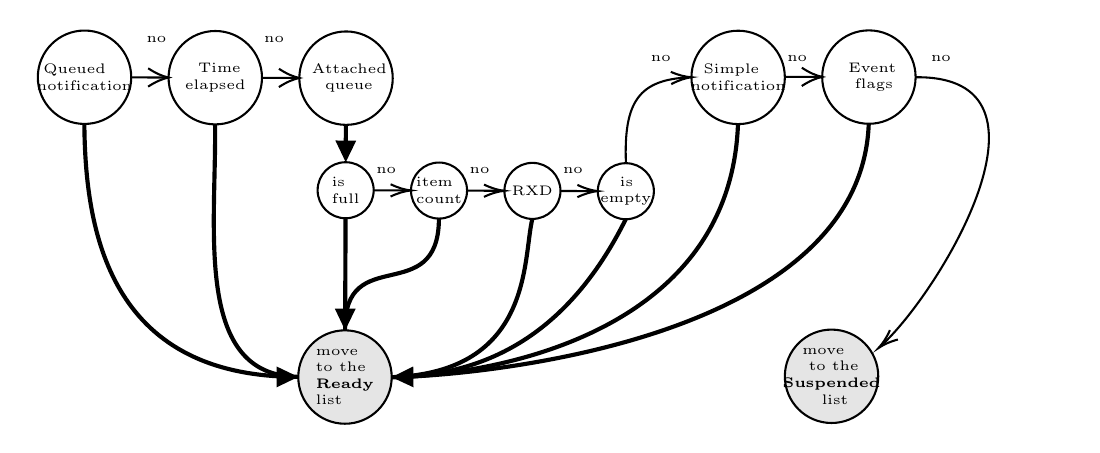
\begin{tikzpicture}[x=0.75pt,y=0.75pt,yscale=-0.9,xscale=0.9]
        \draw   (85.09,90) .. controls (71.28,89.95) and (60.05,101.11) .. (60,114.91) .. controls (59.95,128.72) and (71.11,139.95) .. (84.91,140) .. controls (98.72,140.05) and (109.95,128.89) .. (110,115.09) .. controls (110.05,101.28) and (98.89,90.05) .. (85.09,90) -- cycle ;
        \draw   (155.09,90.24) .. controls (141.28,90.2) and (130.05,101.35) .. (130,115.16) .. controls (129.95,128.96) and (141.11,140.2) .. (154.91,140.24) .. controls (168.72,140.29) and (179.95,129.14) .. (180,115.33) .. controls (180.05,101.52) and (168.89,90.29) .. (155.09,90.24) -- cycle ;
        \draw    (110,115.09) -- (128,115.15) ;
        \draw [shift={(130,115.16)}, rotate = 180.2] [color={rgb, 255:red, 0; green, 0; blue, 0 }  ][line width=0.75]    (10.93,-4.9) .. controls (6.95,-2.3) and (3.31,-0.67) .. (0,0) .. controls (3.31,0.67) and (6.95,2.3) .. (10.93,4.9)   ;
        \draw   (224.84,160.49) .. controls (216.56,160.46) and (209.82,167.15) .. (209.79,175.44) .. controls (209.76,183.72) and (216.45,190.46) .. (224.74,190.49) .. controls (233.02,190.52) and (239.76,183.82) .. (239.79,175.54) .. controls (239.82,167.26) and (233.13,160.52) .. (224.84,160.49) -- cycle ;
        \draw [line width=1.5]    (84.91,140) .. controls (85.37,197.92) and (98.51,274.01) .. (196.45,275.38) ;
        \draw [shift={(199.44,275.4)}, rotate = 539.9200000000001] [fill={rgb, 255:red, 0; green, 0; blue, 0 }  ][line width=0.08]  [draw opacity=0] (11.61,-5.58) -- (0,0) -- (11.61,5.58) -- cycle    ;
        \draw   (225.09,90.49) .. controls (211.28,90.44) and (200.05,101.59) .. (200,115.4) .. controls (199.95,129.21) and (211.1,140.44) .. (224.91,140.49) .. controls (238.72,140.54) and (249.95,129.38) .. (250,115.58) .. controls (250.05,101.77) and (238.89,90.54) .. (225.09,90.49) -- cycle ;
        \draw    (180,115.33) -- (198,115.39) ;
        \draw [shift={(200,115.4)}, rotate = 180.2] [color={rgb, 255:red, 0; green, 0; blue, 0 }  ][line width=0.75]    (10.93,-4.9) .. controls (6.95,-2.3) and (3.31,-0.67) .. (0,0) .. controls (3.31,0.67) and (6.95,2.3) .. (10.93,4.9)   ;
        \draw [line width=1.5]    (224.91,140.49) -- (224.86,156.49) ;
        \draw [shift={(224.84,160.49)}, rotate = 270.2] [fill={rgb, 255:red, 0; green, 0; blue, 0 }  ][line width=0.08]  [draw opacity=0] (11.61,-5.58) -- (0,0) -- (11.61,5.58) -- cycle    ;
        \draw   (274.84,160.66) .. controls (266.56,160.63) and (259.82,167.33) .. (259.79,175.61) .. controls (259.76,183.89) and (266.45,190.63) .. (274.74,190.66) .. controls (283.02,190.69) and (289.76,184) .. (289.79,175.72) .. controls (289.82,167.43) and (283.13,160.69) .. (274.84,160.66) -- cycle ;
        \draw    (239.79,175.54) -- (257.79,175.6) ;
        \draw [shift={(259.79,175.61)}, rotate = 180.2] [color={rgb, 255:red, 0; green, 0; blue, 0 }  ][line width=0.75]    (10.93,-3.29) .. controls (6.95,-1.4) and (3.31,-0.3) .. (0,0) .. controls (3.31,0.3) and (6.95,1.4) .. (10.93,3.29)   ;
        \draw   (324.84,160.84) .. controls (316.56,160.81) and (309.82,167.5) .. (309.79,175.79) .. controls (309.76,184.07) and (316.45,190.81) .. (324.74,190.84) .. controls (333.02,190.87) and (339.76,184.17) .. (339.79,175.89) .. controls (339.82,167.61) and (333.13,160.87) .. (324.84,160.84) -- cycle ;
        \draw [line width=1.5]    (224.74,190.49) -- (224.54,246.49) ;
        \draw [shift={(224.53,250.49)}, rotate = 270.2] [fill={rgb, 255:red, 0; green, 0; blue, 0 }  ][line width=0.08]  [draw opacity=0] (11.61,-5.58) -- (0,0) -- (11.61,5.58) -- cycle    ;
        \draw  [fill=gray!20  ,fill opacity=1 ] (224.53,250.49) .. controls (210.72,250.44) and (199.49,261.59) .. (199.44,275.4) .. controls (199.39,289.21) and (210.55,300.44) .. (224.35,300.49) .. controls (238.16,300.54) and (249.39,289.38) .. (249.44,275.57) .. controls (249.49,261.77) and (238.33,250.54) .. (224.53,250.49) -- cycle ;
        \draw   (435,90.09) .. controls (421.19,90.04) and (409.96,101.19) .. (409.91,115) .. controls (409.86,128.81) and (421.02,140.04) .. (434.83,140.09) .. controls (448.63,140.14) and (459.86,128.98) .. (459.91,115.17) .. controls (459.96,101.37) and (448.81,90.14) .. (435,90.09) -- cycle ;
        \draw    (289.79,175.72) -- (297.46,175.74) -- (307.79,175.78) ;
        \draw [shift={(309.79,175.79)}, rotate = 180.2] [color={rgb, 255:red, 0; green, 0; blue, 0 }  ][line width=0.75]    (10.93,-3.29) .. controls (6.95,-1.4) and (3.31,-0.3) .. (0,0) .. controls (3.31,0.3) and (6.95,1.4) .. (10.93,3.29)   ;
        \draw [line width=1.5]    (154.91,140.24) .. controls (155.5,197) and (143.5,275) .. (199.44,275.4) ;
        \draw [line width=1.5]    (274.74,190.66) .. controls (274.5,239) and (223.5,203) .. (224.53,250.49) ;
        \draw [line width=1.5]    (324.74,190.84) .. controls (319.5,212) and (325.5,273) .. (249.44,275.57) ;
        \draw   (374.84,161.01) .. controls (366.56,160.98) and (359.82,167.68) .. (359.79,175.96) .. controls (359.76,184.24) and (366.45,190.98) .. (374.74,191.01) .. controls (383.02,191.04) and (389.76,184.35) .. (389.79,176.06) .. controls (389.82,167.78) and (383.13,161.04) .. (374.84,161.01) -- cycle ;
        \draw    (339.79,175.89) -- (357.79,175.95) ;
        \draw [shift={(359.79,175.96)}, rotate = 180.2] [color={rgb, 255:red, 0; green, 0; blue, 0 }  ][line width=0.75]    (10.93,-3.29) .. controls (6.95,-1.4) and (3.31,-0.3) .. (0,0) .. controls (3.31,0.3) and (6.95,1.4) .. (10.93,3.29)   ;
        \draw [line width=1.5]    (374.74,191.01) .. controls (342.17,256.37) and (296.35,273.96) .. (253.42,275.48) ;
        \draw [shift={(249.44,275.57)}, rotate = 359.25] [fill={rgb, 255:red, 0; green, 0; blue, 0 }  ][line width=0.08]  [draw opacity=0] (11.61,-5.58) -- (0,0) -- (11.61,5.58) -- cycle    ;
        \draw    (374.84,161.01) .. controls (373.53,127.68) and (382.14,116.45) .. (408.29,115.07) ;
        \draw [shift={(409.91,115)}, rotate = 537.9100000000001] [color={rgb, 255:red, 0; green, 0; blue, 0 }  ][line width=0.75]    (10.93,-3.29) .. controls (6.95,-1.4) and (3.31,-0.3) .. (0,0) .. controls (3.31,0.3) and (6.95,1.4) .. (10.93,3.29)   ;
        \draw   (505,89.91) .. controls (491.19,89.86) and (479.96,101.02) .. (479.91,114.83) .. controls (479.86,128.63) and (491.02,139.86) .. (504.83,139.91) .. controls (518.63,139.96) and (529.86,128.81) .. (529.91,115) .. controls (529.96,101.19) and (518.81,89.96) .. (505,89.91) -- cycle ;
        \draw    (459.91,114.76) -- (477.91,114.82) ;
        \draw [shift={(479.91,114.83)}, rotate = 180.2] [color={rgb, 255:red, 0; green, 0; blue, 0 }  ][line width=0.75]    (10.93,-4.9) .. controls (6.95,-2.3) and (3.31,-0.67) .. (0,0) .. controls (3.31,0.67) and (6.95,2.3) .. (10.93,4.9)   ;
        \draw [line width=1.5]    (434.83,140.09) .. controls (430.5,257) and (293.5,275) .. (249.44,275.57) ;
        \draw [line width=1.5]    (504.83,139.91) .. controls (500.5,256.83) and (293.5,275) .. (249.44,275.57) ;
        \draw  [fill=gray!20 ] (485,250.09) .. controls (471.19,250.04) and (459.96,261.19) .. (459.91,275) .. controls (459.86,288.81) and (471.02,300.04) .. (484.83,300.09) .. controls (498.63,300.14) and (509.86,288.98) .. (509.91,275.17) .. controls (509.96,261.37) and (498.81,250.14) .. (485,250.09) -- cycle ;
        \draw    (529.91,115) .. controls (613.23,114.01) and (542.77,230.26) .. (511.41,258.76) ;
        \draw [shift={(510,260)}, rotate = 319.45] [color={rgb, 255:red, 0; green, 0; blue, 0 }  ][line width=0.75]    (10.93,-3.29) .. controls (6.95,-1.4) and (3.31,-0.3) .. (0,0) .. controls (3.31,0.3) and (6.95,1.4) .. (10.93,3.29)   ;
        \draw (85,115) node  [font=\tiny] [align=left] { \ Queued\\notification};
        \draw (224.79,175.49) node  [font=\tiny] [align=left] {is\\full};
        \draw (274.79,175.66) node  [font=\tiny] [align=left] {item\\count};
        \draw (324.79,175.84) node  [font=\tiny] [align=left] {RXD};
        \draw (224.44,275.49) node  [font=\tiny] [align=left] {move \\to the\\\textbf{Ready} \\list};
        \draw (374.79,176.01) node  [font=\tiny] [align=left] { \ \ \ is\\empty};
        \draw (155,115.24) node  [font=\tiny] [align=left] { \ \ Time\\elapsed};
        \draw (225,115.49) node  [font=\tiny] [align=left] { \ Attached\\ \ \ \ queue};
        \draw (434.91,115.09) node  [font=\tiny] [align=left] { \ \ Simple\\notification};
        \draw (504.91,114.91) node  [font=\tiny] [align=left] { \ Event\\ \ \ flags};
        \draw (484.91,275.09) node  [font=\tiny] [align=left] { \ \ \ move \\ \ \ \ \ to the\\\textbf{Suspended} \\ \ \ \ \ \ \ list};
        \draw (123.5,95) node  [font=\tiny] [align=left] {no};
        \draw (186.5,95) node  [font=\tiny] [align=left] {no};
        \draw (246.5,165) node  [font=\tiny] [align=left] {no};
        \draw (296.5,165) node  [font=\tiny] [align=left] {no};
        \draw (346.5,165) node  [font=\tiny] [align=left] {no};
        \draw (393.5,105) node  [font=\tiny] [align=left] {no};
        \draw (466.5,105) node  [font=\tiny] [align=left] {no};
        \draw (543.5,105) node  [font=\tiny] [align=left] {no};
    \end{tikzpicture}
    \caption{Event precedence}
    \label{fig:eventprecedence}
\end{figure}

\paragraph{Additional operational states :}
Each task has independent operating states from those globally controlled by the scheduler. These states can be handled by the application writer to modify the event-flow to the task and consequently, affecting the transition to the \textit{qReady} global state. These states are described below.

\begin{itemize}
    \item \textit{qAwake} : In this state, the task is conceptually in an alert mode, handling most of the available events. This operational state is available when the \lstinline{SHUTDOWN} bit is set, allowing the next operational states to be available:
    \begin{itemize}
        \item \textit{qEnabled} : The task is able to catch all the events. This operational state is available when the \lstinline{ENABLE} bit is set.
        \item \textit{qDisabled} : In this state the time events will be discarded. This operational state is available when the \lstinline{ENABLE} bit is cleared.
    \end{itemize}
    \item \textit{qAsleep} : Task operability is put into a deep doze mode, so the task can't be triggered by the lower precedence events.  This operational state is available when the \lstinline{SHUTDOWN} bit is cleared. The task can exit from this operational state when it receives a high precedence event (a queued notification) or using the \lstinline{qTask_Set_State()} API.
\end{itemize}

The figure \ref{fig:eventflow} shows a better representation of how the event flow can be affected by this operational states.

\begin{tcolorbox}
\HandRight Queued notifications are the only event that can wake up sleeping tasks.
\end{tcolorbox}
\begin{tcolorbox}
\HandRight The \textit{qAsleep} operational state overrides the \textit{qEnabled} and \textit{qDisabled} State.
\end{tcolorbox}

\begin{figure}[H]
    \centering
    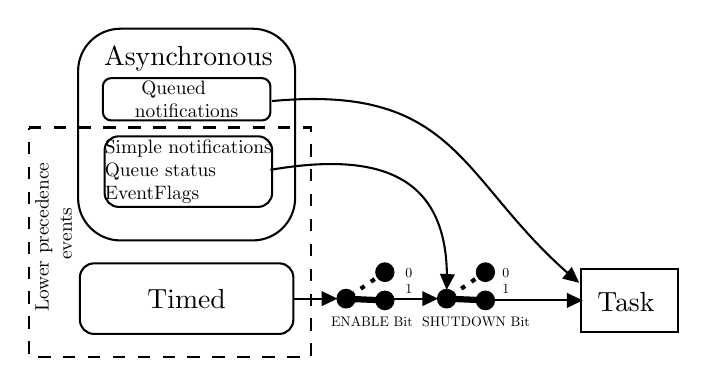
\begin{tikzpicture}[x=0.75pt,y=0.75pt,yscale=-0.85,xscale=0.85]
        \draw   (41.5,194) .. controls (41.5,189.58) and (45.08,186) .. (49.5,186) -- (154.5,186) .. controls (158.92,186) and (162.5,189.58) .. (162.5,194) -- (162.5,218) .. controls (162.5,222.42) and (158.92,226) .. (154.5,226) -- (49.5,226) .. controls (45.08,226) and (41.5,222.42) .. (41.5,218) -- cycle ;
        \draw   (40.5,77) .. controls (40.5,63.75) and (51.25,53) .. (64.5,53) -- (139.5,53) .. controls (152.75,53) and (163.5,63.75) .. (163.5,77) -- (163.5,149) .. controls (163.5,162.25) and (152.75,173) .. (139.5,173) -- (64.5,173) .. controls (51.25,173) and (40.5,162.25) .. (40.5,149) -- cycle ;
        \draw   (55.5,122) .. controls (55.5,117.58) and (59.08,114) .. (63.5,114) -- (142.5,114) .. controls (146.92,114) and (150.5,117.58) .. (150.5,122) -- (150.5,146) .. controls (150.5,150.42) and (146.92,154) .. (142.5,154) -- (63.5,154) .. controls (59.08,154) and (55.5,150.42) .. (55.5,146) -- cycle ;
        \draw   (325.5,189) -- (380.5,189) -- (380.5,225) -- (325.5,225) -- cycle ;
        \draw [line width=2.25]    (214.38,207) -- (191,206) ;
        \draw  [fill={rgb, 255:red, 0; green, 0; blue, 0 }  ,fill opacity=1 ] (187.5,206) .. controls (187.5,203.24) and (189.68,201) .. (192.38,201) .. controls (195.07,201) and (197.25,203.24) .. (197.25,206) .. controls (197.25,208.76) and (195.07,211) .. (192.38,211) .. controls (189.68,211) and (187.5,208.76) .. (187.5,206) -- cycle ;
        \draw    (324.5,207) -- (276.25,207) ;
        \draw [shift={(326.5,207)}, rotate = 180] [fill={rgb, 255:red, 0; green, 0; blue, 0 }  ][line width=0.75]  [draw opacity=0] (8.93,-4.29) -- (0,0) -- (8.93,4.29) -- cycle    ;
        \draw  [fill={rgb, 255:red, 0; green, 0; blue, 0 }  ,fill opacity=1 ] (209.5,191) .. controls (209.5,188.24) and (211.68,186) .. (214.38,186) .. controls (217.07,186) and (219.25,188.24) .. (219.25,191) .. controls (219.25,193.76) and (217.07,196) .. (214.38,196) .. controls (211.68,196) and (209.5,193.76) .. (209.5,191) -- cycle ;
        \draw  [fill={rgb, 255:red, 0; green, 0; blue, 0 }  ,fill opacity=1 ] (209.5,207) .. controls (209.5,204.24) and (211.68,202) .. (214.38,202) .. controls (217.07,202) and (219.25,204.24) .. (219.25,207) .. controls (219.25,209.76) and (217.07,212) .. (214.38,212) .. controls (211.68,212) and (209.5,209.76) .. (209.5,207) -- cycle ;
        \draw    (185.5,206) -- (162.5,206) ;
        \draw [shift={(187.5,206)}, rotate = 180] [fill={rgb, 255:red, 0; green, 0; blue, 0 }  ][line width=0.75]  [draw opacity=0] (8.93,-4.29) -- (0,0) -- (8.93,4.29) -- cycle    ;
        \draw  [fill={rgb, 255:red, 0; green, 0; blue, 0 }  ,fill opacity=1 ] (244.5,206) .. controls (244.5,203.24) and (246.68,201) .. (249.38,201) .. controls (252.07,201) and (254.25,203.24) .. (254.25,206) .. controls (254.25,208.76) and (252.07,211) .. (249.38,211) .. controls (246.68,211) and (244.5,208.76) .. (244.5,206) -- cycle ;
        \draw  [fill={rgb, 255:red, 0; green, 0; blue, 0 }  ,fill opacity=1 ] (266.5,191) .. controls (266.5,188.24) and (268.68,186) .. (271.38,186) .. controls (274.07,186) and (276.25,188.24) .. (276.25,191) .. controls (276.25,193.76) and (274.07,196) .. (271.38,196) .. controls (268.68,196) and (266.5,193.76) .. (266.5,191) -- cycle ;
        \draw  [color={rgb, 255:red, 0; green, 0; blue, 0 }  ,draw opacity=1 ][fill={rgb, 255:red, 0; green, 0; blue, 0 }  ,fill opacity=1 ] (266.5,207) .. controls (266.5,204.24) and (268.68,202) .. (271.38,202) .. controls (274.07,202) and (276.25,204.24) .. (276.25,207) .. controls (276.25,209.76) and (274.07,212) .. (271.38,212) .. controls (268.68,212) and (266.5,209.76) .. (266.5,207) -- cycle ;
        \draw    (242.5,206) -- (219.5,206) ;
        \draw [shift={(244.5,206)}, rotate = 180] [fill={rgb, 255:red, 0; green, 0; blue, 0 }  ][line width=0.75]  [draw opacity=0] (8.93,-4.29) -- (0,0) -- (8.93,4.29) -- cycle    ;
        \draw    (149.5,133) .. controls (212.86,122.11) and (251.72,136.7) .. (249.46,199.09) ;
        \draw [shift={(249.38,201)}, rotate = 272.8] [fill={rgb, 255:red, 0; green, 0; blue, 0 }  ][line width=0.75]  [draw opacity=0] (8.93,-4.29) -- (0,0) -- (8.93,4.29) -- cycle    ;
        \draw   (54.5,85.8) .. controls (54.5,83.15) and (56.65,81) .. (59.3,81) -- (144.7,81) .. controls (147.35,81) and (149.5,83.15) .. (149.5,85.8) -- (149.5,100.2) .. controls (149.5,102.85) and (147.35,105) .. (144.7,105) -- (59.3,105) .. controls (56.65,105) and (54.5,102.85) .. (54.5,100.2) -- cycle ;
        \draw    (150.5,94) .. controls (257.96,84.05) and (256.52,140.43) .. (323.49,196.16) ;
        \draw [shift={(324.5,197)}, rotate = 219.47] [fill={rgb, 255:red, 0; green, 0; blue, 0 }  ][line width=0.75]  [draw opacity=0] (8.93,-4.29) -- (0,0) -- (8.93,4.29) -- cycle    ;
        \draw  [dash pattern={on 4.5pt off 4.5pt}] (12.5,109) -- (172.5,109) -- (172.5,239) -- (12.5,239) -- cycle ;
        \draw [line width=2.25]    (272.75,207) -- (249.38,206) ;
        \draw [line width=1.5]  [dash pattern={on 1.69pt off 2.76pt}]  (214.38,191) -- (192.38,206) ;
        \draw [line width=1.5]  [dash pattern={on 1.69pt off 2.76pt}]  (271.38,191) -- (249.38,206) ;
        \draw (102,206) node  [align=left] {Timed};
        \draw (103,70) node  [align=left] {Asynchronous};
        \draw (351,208) node  [align=left] {Task};
        \draw (103,134) node [scale=0.7] [align=left] {Simple notifications\\Queue status\\EventFlags};
        \draw (102,93) node [scale=0.7] [align=left] { \ Queued \\notifications};
        \draw (207,219) node [scale=0.5] [align=left] {ENABLE Bit};
        \draw (266,219) node [scale=0.5] [align=left] {SHUTDOWN Bit};
        \draw (26.5,171) node [scale=0.7,rotate=-270] [align=left] {Lower precedence\\ \ \ \ \ \ \ \ \ events};
        \draw (228,196) node [scale=0.5] [align=left] {0\\1};
        \draw (283,196) node [scale=0.5] [align=left] {0\\1};
    \end{tikzpicture}
    \caption{Event flow according operational states}
    \label{fig:eventflow}
\end{figure}


\subsection{Getting started}
Unpack the source files and copy them into your project. Also, add a copy of the file \lstinline{qconfig.h} and modify it according to your needs. Setup your compiler include path with the corresponding OS directory. Include the header file \lstinline{QuarkTS.h} and setup the instance of the kernel using the \lstinline{qOS_Setup()} inside the main thread. Additional configuration to the target compiler may be required to add the path to the directory of header files. The code below shows a common initialization in the main source file.
\medskip

File: \lstinline{main.c}
\lstinputlisting[style=CStyle]{sec1gettingstarted.c}


In the above code, the following considerations should be taken
\begin{itemize}
    \item The function \lstinline{qOS_Setup()} must be called before any interaction with the OS.
    \item The procedure \lstinline{HardwareSetup()} should be a function with all the hardware instructions needed to initialize the target system.
    \item  The procedure \lstinline{Configure_Periodic_Timer_Interrupt_1ms()} should be a function with all the hardware instructions needed to initialize and run a timer with an overflow tick of one millisecond.
\end{itemize}

Tasks can be later added to the scheduling scheme by simply calling \lstinline{qOS_Add_Task()} or any of the other available APIs for specific purpose tasks.

\subsection{Recommended programming pattern}
A multitasking design pattern demands a better project organization. To have this attribute in your solution, code the tasks in a separate source file. A simple implementation example is presented below.
\medskip

To make the handling of the tasks available in other contexts, nodes should be globals(see the \lstinline{extern} qualifier in \lstinline{MyAppTasks.h} header file).  Avoid implementing functionalities in a component that are not related to each other. Put any other components and globals resources in a separated source file, for example (\lstinline{ScreenDriver.h}/\lstinline{ScreenDriver.c}),  (\lstinline{Globals.h}/\lstinline{Globals.c}). These simple design tips will allow you to have a better principle of abstraction and will maximize the cohesion of the solution, improving the code readability and maintenance.
\medskip

File: \lstinline{MyAppTasks.h}
\lstinputlisting[style=CStyle]{MyAppTasks.h}

File: \lstinline{MyAppTasks.c}
\lstinputlisting[style=CStyle]{MyAppTasks.c}

File: \lstinline{main.c}
\lstinputlisting[style=CStyle]{sec1recpattern.c}


\subsection{Critical sections}
Since the kernel is non-preemptive, the only critical section that must be handled are the shared resources accessed from the ISR context. Perhaps, the most obvious way of achieving mutual exclusion is to allow the kernel to disable interrupts before it enters its critical section and then, enable interrupts after it leaves its critical section. 
\medskip

By disabling interrupts, the CPU will be unable to change the current context. This guarantees that the currently running job can use a shared resource without another context accessing it. But, disabling interrupts, is a major undertaking. At best, the system will not be able to service interrupts for the time the current job is doing in its critical section, however, in QuarkTS, these critical sections are handled as quickly as possible.  

Considering that the kernel is hardware-independent, the application writer should provide the necessary piece of code to enable and disable interrupts.

For this, the \lstinline{qCritical_SetInterruptsED()} \index{\lstinline{qCritical_SetInterruptsED}} API should be used. In this way, communication between ISR and tasks using queued notifications or data queues is performed safely. 
\medskip

\begin{lstlisting}[style=CStyle]
void qCritical_SetInterruptsED( void (*Restorer)(qUINT32_t), 
                                qUINT32_t (*Disabler)(void) );
\end{lstlisting}

\subsubsection*{Parameters:}
\begin{itemize}
    \item \lstinline{Restorer} : The function with hardware specific code to enable or restore interrupts.
    \item \lstinline{Disabler} : The function with hardware specific code that disables interrupts.
\end{itemize}

In some systems, disabling the global IRQ flags is not enough, as they don't save/restore state of interrupt, so here, the \lstinline{qUINT32_t} argument and return value in both functions (\lstinline{Disabler} and \lstinline{Restorer}) becomes relevant, because they can be used by the application writer to save and restore the current interrupt configuration. So, when a critical section is performed, the \lstinline{Disabler}, in addition to disable the interrupts, return the current configuration to be retained by the kernel, later when the critical section finish, this retained value is passed to \lstinline{Restorer} to bring back the saved configuration. 

\subsection{Task management APIs in run-time }
Most of the scheduling parameters regarding task execution can be changed at run-time. The following APIs are intended for this purpose. 
\medskip


\begin{lstlisting}[style=CStyle]
void qTask_Set_Time( qTask_t * const Task, const qTime_t Value )
\end{lstlisting}

Set/Change the task execution interval. \index{\lstinline{qTask_Set_Time}}

\subsubsection*{Parameters:}
\begin{itemize}
    \item \lstinline{Task} : A pointer to the task node.
    \item \lstinline{Value} : Execution interval defined in seconds (floating-point format). For immediate execution use \lstinline{qTimeImmediate}.
\end{itemize}

\noindent\hrulefill

\begin{lstlisting}[style=CStyle]
void qTask_Set_Iterations( qTask_t * const Task, qIteration_t Value )
\end{lstlisting}

Set/Change the number of task iterations. \index{\lstinline{qTask_Set_Iterations}}

\subsubsection*{Parameters:}
\begin{itemize}
    \item \lstinline{Task} : A pointer to the task node.
    \item \lstinline{Value} : Number of task executions (integer value). For indefinite execution user \lstinline{qPeriodic} or \lstinline{qIndefinite}. Tasks do not remember the number of iteration set initially. 
\end{itemize}

\noindent\hrulefill


\begin{lstlisting}[style=CStyle]
void qTask_Set_Priority( qTask_t * const Task, qPriority_t Value )
\end{lstlisting}

Set/Change the task priority value. \index{\lstinline{qTask_Set_Priority}}

\subsubsection*{Parameters:}
\begin{itemize}
    \item \lstinline{Task} : A pointer to the task node.
    \item \lstinline{Value} : Priority value. \lstinline{[0(min) - Q_PRIORITY_LEVELS(max)]}. 
\end{itemize}

\noindent\hrulefill


\begin{lstlisting}[style=CStyle]
void qTask_Set_Callback( qTask_t * const Task, qTaskFcn_t CallbackFcn )
\end{lstlisting}

Set/Change the task callback function. \index{\lstinline{qTask_Set_Callback}}. Can be used to detach an state machine.

\subsubsection*{Parameters:}
\begin{itemize}
    \item \lstinline{Task} : A pointer to the task node.
    \item \lstinline{Callback} : A pointer to a void callback method with a \lstinline{qEvent_t} parameter as input argument.
\end{itemize}

\noindent\hrulefill


\begin{lstlisting}[style=CStyle]
void qTask_Set_State( qTask_t * const Task, const qState_t State ) 
void qTask_Resume( qTask_t * const Task ) 
void qTask_Suspend( qTask_t * const Task )
void qTask_ASleep( qTask_t * const Task )
void qTask_Awake( qTask_t * const Task )
\end{lstlisting}\index{\lstinline{qTask_Resume}} \index{\lstinline{qTask_Suspend}} \index{\lstinline{qTask_ASleep}} \index{\lstinline{qTask_Awake}}

Set the task operability state. \index{\lstinline{qTask_Set_State}} \index{\lstinline{qTask_Resume}} \index{\lstinline{qTask_Suspend}}

\subsubsection*{Parameters:}
\begin{itemize}
    \item \lstinline{Task} : A pointer to the task node.
    \item \lstinline{State} : Use one of the following values:
    \begin{itemize}
        \item \lstinline{qEnabled} : Task will be able to catch all the events.
        \item \lstinline{qDisabled} : Time events will be ignored. Only asynchronous events are allowed.
        \item \lstinline{qAsleep} : The task can't be triggered by lower precedence events. Only the queued notifications events can be caught.
        \item \lstinline{qAwake} : Task will be able to catch all the events.
    \end{itemize}
\end{itemize}

\noindent\hrulefill


\begin{lstlisting}[style=CStyle]
void qTask_Set_Data( qTask_t * const Task, void* UserData )
\end{lstlisting}

Set the task data. \index{\lstinline{qTask_Set_Data}}

\subsubsection*{Parameters:}
\begin{itemize}
    \item \lstinline{Task} : A pointer to the task node.
    \item \lstinline{UserData} : A pointer to the associated data.
\end{itemize}

\noindent\hrulefill


\begin{lstlisting}[style=CStyle]
void qTask_ClearTimeElapsed( qTask_t * const Task )
\end{lstlisting}

Clear the elapsed time of the task. Restart the internal task tick. \index{\lstinline{qTask_ClearTimeElapsed}}

\subsubsection*{Parameters:}
\begin{itemize}
    \item \lstinline{Task} : A pointer to the task node.
\end{itemize}

\noindent\hrulefill


\begin{lstlisting}[style=CStyle]
qCycles_t qTask_Get_Cycles( const qTask_t * const Task )
\end{lstlisting}

Retrieve the number of task activation's. \index{\lstinline{qTask_Get_Cycles}}

\subsubsection*{Parameters:}
\begin{itemize}
    \item \lstinline{Task} : A pointer to the task node.
\end{itemize}


\subsubsection*{Return value:}
A \lstinline{qUINT32_t} value containing the number of task activations.

\noindent\hrulefill

\begin{lstlisting}[style=CStyle]
qState_t qTask_Get_State( const qTask_t * const Task )
\end{lstlisting}

Retrieve the task operational state. \index{\lstinline{qTask_Get_State}}

\subsubsection*{Parameters:}
\begin{itemize}
    \item \lstinline{Task} : A pointer to the task node.
\end{itemize}

\subsubsection*{Return value:}
\lstinline{qEnabled} or \lstinline{qDisabled} if the task is \lstinline{qAwaken}. \lstinline{qAsleep} if the task is in a sleep operational state.

\noindent\hrulefill


\begin{lstlisting}[style=CStyle]
qTask_t* qTask_Self( void )
\end{lstlisting}

Get current running task handle. \index{\lstinline{qTask_Self}}

\subsubsection*{Return value:}
A pointer to the current running task. \lstinline{NULL} when the scheduler it's in a busy state or when idle-task is running.


\noindent\hrulefill


\begin{lstlisting}[style=CStyle]
qTask_GlobalState_t qTask_Get_GlobalState( const qTask_t * const Task )
\end{lstlisting}

Retrieve the task global-state. \index{\lstinline{qTask_Get_GlobalState}}

\subsubsection*{Parameters:}
\begin{itemize}
    \item \lstinline{Task} : A pointer to the task node.
\end{itemize}


\subsubsection*{Return value:}
One of the available global states : \lstinline{qWaiting}, \lstinline{qSuspended}, \lstinline{qRunning} or \lstinline{qReady}.
Return \lstinline{qUndefinedGlobalState} if the current task its passing through a current kernel transaction

\noindent\hrulefill

\begin{lstlisting}[style=CStyle]
qBool_t qTask_HasPendingNotifications( const qTask_t * const Task  )
\end{lstlisting}

Check if the task has pending notifications. Please read section \ref{osnotifications}. \index{\lstinline{qTask_HasPendingNotifications}}

\subsubsection*{Parameters:}
\begin{itemize}
    \item \lstinline{Task} : A pointer to the task node.
\end{itemize}

\subsubsection*{Return value:}
\lstinline{qTrue} if the functon asserts, otherwise returns \lstinline{qFalse}.

\subsection{Demonstrative examples}
\subsubsection{A simple scheduling}
This example demonstrates a simple environment setup for multiple tasks. Initially, only \lstinline{task1} and \lstinline{task2} are enabled. \lstinline{task1} runs every 2 seconds 10 times and then stops. \lstinline{task2} runs every 3 seconds indefinitely. \lstinline{task1} enables \lstinline{task3} at its first run. \lstinline{task3} run every 5 seconds. \lstinline{task1} disables \lstinline{task3} on its last iteration and changed \lstinline{task2} to run every 1/2 seconds. In the end, \lstinline{task2} is the only task running every 1/2 seconds.
\medskip

\lstinputlisting[style=CStyle]{sec1demosimple.c}

\subsubsection{Using the task argument}
As seen in section \ref{addtask}, tasks can accept a parameter of type pointer to void (\lstinline{void*}). 
This parameter could be used for multiple applications, including storage, task identification, duplication removal and others. The following example shows the usage of this argument to avoid callback duplication among tasks with the same behavior. 

Consider a scenario where you have to build a digital controller for many physical variables, for example, a PID controller for temperature, humidity and light. The PID algorithm will be the same for all variables. The only difference will be the variable input, the controlled output action and the PID gains. In this case, each of the PID tasks will utilize the same callback methods. The only difference will be the I/O parameters (specific for each PID controller). 
\medskip

Let's define a PID data structure with the I/O variables and gains.
\medskip
 
\lstinputlisting[style=CStyle]{sec1demo2def.c}

A task will be added to the scheme to collect the sensor data and apply the respective control output. 
\medskip

\begin{lstlisting}[style=CStyle]
qOS_Add_Task( &IO_TASK, IO_TASK_Callback, qMedium_Priority, 0.1, qPeriodic, 
              qEnabled, "iotask");
\end{lstlisting}

\lstinputlisting[style=CStyle]{sec1demo2iotask.c}

Then, three different tasks are created to apply the respective PID controller. Note that these tasks refer to the same callback methods and we assign pointers to the respective variables. 
\medskip

\lstinputlisting[style=CStyle]{sec1demo2addtasks.c}

\lstinputlisting[style=CStyle]{sec1demo2pidtask.c}

\newpage

\subsection{Configuration macros}
Some  OS features can be customized using a set of macros located in the header file \lstinline{qconfig.h}. Here is the default configuration, followed by an explanation of each macro: 
\medskip

\begin{adjustbox}{width=\textwidth,totalheight={18cm}}
\begin{tabularx}
{\textwidth}{l X}
\hline
{\lstinline!Q_PRIORITY_LEVELS!} & \textit{Default:} {\lstinline!3!}.  The number of priorities available for application tasks.\\
\hline
{\lstinline!Q_SETUP_TIME_CANONICAL!} & \textit{Default:}
{\lstinline!0(disabled)!}. If enabled, the kernel assumes the timing base to 1mS(1KHz). So all time specifications for tasks and STimers must be set in milliseconds(mS). Also can be used to remove the floating-point operations when dealing with time. In some systems, can reduce the memory usage. \\
\hline
{\lstinline!Q_SETUP_TICK_IN_HERTZ!} & \textit{Default:} {\lstinline!0(disabled)!}. If enabled, the timing base will be taken as frequency(Hz) instead of period(S) by {\lstinline!qOS_Setup()!} (In some systems, can reduce the memory usage ). \\
\hline
{\lstinline!Q_PRIO_QUEUE_SIZE!} & \textit{Default:} {\lstinline!10!}.  Size of the priority queue for notifications. This argument should be an integer number greater than zero. A zero value can be used to disable this functionality.\\
\hline
{\lstinline!Q_PRESERVE_TASK_ENTRY_ORDER !} & \textit{Default:} {\lstinline!0(disabled)!}. If enabled, kernel will preserve the tasks entry order every OS scheduling cycle.\\
\hline
{\lstinline!Q_MEMORY_MANAGER!} & \textit{Default:} {\lstinline!1(enabled)!}. Used to enable or disable the memory management module. \\
\hline
{\lstinline!Q_BYTE_ALIGNMENT!} & \textit{Default:} {\lstinline!8!}. Used by the memory management module to perform the byte-alignment. \\
\hline
{\lstinline!Q_DEFAULT_HEAP_SIZE!} & \textit{Default:} {\lstinline!2048!}. The total amount of heap size for the default memory pool. \\
\hline
{\lstinline!Q_NOTIFICATION_SPREADER!} & \textit{Default:} {\lstinline!0(disabled)!}. Used to enable or disable the spread notification functionality. \\
\hline
{\lstinline!Q_FSM!} & \textit{Default:} {\lstinline!1(enabled)!}.  Used to enable or disable the Finite State Machine (FSM) extension. \\
\hline
{\lstinline!Q_FSM_MAX_NEST_DEPTH!} & \textit{Default:} {\lstinline!5!}.  The max depth of nesting in Finite State Machines (FSM). \\
\hline
{\lstinline!Q_FSM_MAX_TIMEOUTS!} & \textit{Default:} {\lstinline!3!}.  Max number of timeouts inside a timeout specification for the Finite State machine (FSM) module.\\
\hline
{\lstinline!Q_QUEUES!} & \textit{Default:} {\lstinline!1(enabled)!}.  Used to enable or disable the queues APIs for communication to tasks. \\
\hline
{\lstinline!Q_TRACE_VARIABLES!} & \textit{Default:} {\lstinline!1(enabled)!}.  Used to enable or disable  debug and trace macros.\\
\hline
{\lstinline!Q_DEBUGTRACE_BUFSIZE!} & \textit{Default:} {\lstinline!36!}. The buffer size for debug and trace macros.\\
\hline
{\lstinline!Q_DEBUGTRACE_FULL!} & \textit{Default:} {\lstinline!1(enabled)!}. Used to enable of disable the extended output of trace macros.\\
\hline
{\lstinline!Q_ATCLI!} & \textit{Default:} {\lstinline!1(enabled)!}. Used to enable or disable the AT Command Line Interface (CLI) module. \\
\hline
{\lstinline!Q_TASK_COUNT_CYCLES!} & \textit{Default:} {\lstinline!0(disabled)!}. Used to enable or disable the cycle count in tasks. \\
\hline
{\lstinline!Q_TASK_EVENT_FLAGS!} & \textit{Default:} {\lstinline!1(enabled)!}. Used to enable or disable the task event flags.\\
\hline
{\lstinline!Q_MAX_FTOA_PRECISION!} & \textit{Default:} {\lstinline!10!}. The default precision used to perform float to ASCII conversions. \\
\hline
{\lstinline!Q_ATOF_FULL!} & \textit{Default:} {\lstinline!0(disabled)!}. Used to enable or disable the scientific notation in ASCII to float conversions. \\
\hline
{\lstinline!Q_ALLOW_SCHEDULER_RELEASE!} & \textit{Default:} {\lstinline!0(disabled)!}. Used to enable or disable the scheduler release functionality. \\
\hline
{\lstinline!Q_RESPONSE_HANDLER!} & \textit{Default:} {\lstinline!1(enabled)!}. Used to enable or disable the response handler functionality. \\
\hline
{\lstinline!Q_EDGE_CHECK_IOGROUPS!} & \textit{Default:} {\lstinline!1(enabled)!}. Used to enable or disable the edge check functionality for I/O groups . \\
\hline
{\lstinline!Q_BYTE_SIZED_BUFFERS!} & \textit{Default:} {\lstinline!1(enabled)!}. Used to enable or disable the usage of Byte-sized buffers. \\
\hline
{\lstinline!Q_USE_STDINT_H!} & \textit{Default:} {\lstinline!1(enabled)!}. Use the \lstinline{stdint.h} header to define kernel data-types. \\
\hline
\end{tabularx}
\end{adjustbox}

\newpage